\documentclass[12pt,a4paper,bibliography=totocnumbered,listof=totocnumbered]{article}
\usepackage[ngerman]{babel}
\usepackage[utf8]{inputenc}
\usepackage{amsmath}
\usepackage{amsfonts}
\usepackage{amssymb}
\usepackage{graphicx}
\usepackage{fancyhdr}
\usepackage{tabularx}
\usepackage{geometry}
\usepackage{setspace}
\usepackage[right]{eurosym}
\usepackage[printonlyused]{acronym}
\usepackage{subfig}
\usepackage{floatflt}
\usepackage[usenames,dvipsnames]{color}
\usepackage{colortbl}
\usepackage{paralist}
\usepackage{array}
%\usepackage{titlesec}
\usepackage{parskip}
\usepackage[right]{eurosym}
%\usepackage{picins}
\usepackage[subfigure,titles]{tocloft}
\usepackage[pdfpagelabels=true]{hyperref}
\usepackage{float}

\usepackage{listings}
\lstset{basicstyle=\footnotesize, captionpos=b, breaklines=true, showstringspaces=false, tabsize=2, frame=lines, numbers=left, numberstyle=\tiny, xleftmargin=2em, framexleftmargin=2em}
\makeatletter
\def\l@lstlisting#1#2{\@dottedtocline{1}{0em}{1em}{\hspace{1,5em} Lst. #1}{#2}}
\makeatother

\geometry{a4paper, top=27mm, left=20mm, right=20mm, bottom=35mm, headsep=10mm, footskip=12mm}


\hypersetup{unicode=false, pdftoolbar=true, pdfmenubar=true, pdffitwindow=false, pdfstartview={FitH},
	pdftitle={Wahlpflichtfach: Implementierung von Brettspielen am Beispiel ReversiXT (SS \the\year)},
	pdfauthor={Dr.\ Carsten Kern},
	pdfsubject={Projektbericht},
	pdfcreator={\LaTeX\ with package \flqq hyperref\frqq},
	pdfproducer={pdfTeX \the\pdftexversion.\pdftexrevision},
	pdfkeywords={Projektbericht, ReversiXT},
	pdfnewwindow=true,
	colorlinks=true,linkcolor=black,citecolor=black,filecolor=magenta,urlcolor=black}
\pdfinfo{/CreationDate (D:20151500000000)}
%\titlespacing{\section}{0pt}{12pt plus 4pt minus 2pt}{-6pt plus 2pt minus 2pt}

% Kopf- und Fusszeile
\renewcommand{\sectionmark}[1]{\markright{#1}}
\renewcommand{\leftmark}{\rightmark}
\pagestyle{fancy}
\lhead{}
\chead{}
\rhead{\thesection\space\contentsname}
\lfoot{Implementierung von Brettspielen am Beispiel ReversiXT -- SS \the\year}
\cfoot{}
\rfoot{\ \linebreak Seite \thepage}
\renewcommand{\headrulewidth}{0.4pt}
\renewcommand{\footrulewidth}{0.4pt}

% Vorspann
\renewcommand{\thesection}{\Roman{section}}
\renewcommand{\theHsection}{\Roman{section}}
\pagenumbering{Roman}

\newcommand{\folgen}[1]{
\ensuremath
#1
}

\newcommand{\MyTitlepage}[5][\empty]{
\thispagestyle{empty}
\begin{center}
	
\includegraphics[scale=0.2]{pics/oth-logo.png}\\
	\vspace*{2cm}
	\Large
	\textbf{Fakultät}\\
	\textbf{Informatik und Mathematik}\\
	\vspace*{2cm}
	\Huge
	\textbf{Projektbericht}\\
	\vspace*{0.5cm}
	\large
	zum Wahlpflichtfach im SS \the\year\\
	\vspace*{1cm}
	\textbf{Implementierung von Brettspielen am Beispiel ReversiXT}\\
	\vspace*{1cm}
	\includegraphics[height=6cm]{#1}
	\vfill
	\normalsize
	%\newcolumntype{x}[1]{>{\raggedleft\arraybackslash\hspace{0pt}}p{#1}}
	\begin{tabular}{rl}%{6cm}p{7.5cm}}
	    \rule{0mm}{5ex}\textbf{Gruppe:} & #2 \\
		\rule{0mm}{5ex}\textbf{Autoren:} & \hspace*{-0.5em}\begin{tabular}[t]{r}#3\end{tabular} \\ 
		\rule{0mm}{5ex}\textbf{Leiter:} & Prof. Dr. rer. nat. Carsten Kern \\ 
		\rule{0mm}{5ex}\textbf{Abgabedatum:} & #4 \\ 
	\end{tabular} 
\end{center}
\pagebreak
}

\begin{document}

% ----------------------------------------------------------------------------------------------------------
% Titelseite
% ----------------------------------------------------------------------------------------------------------
\MyTitlepage[pics/gamefield02]{05}{
\texttt{robin.jahn@st.oth-regensburg.de}\\
\texttt{simon1.melcher@st.oth-regensburg.de}\\
\texttt{alexander1.wess@st.oth-regensburg.de}}
{??.??.\the\year} % FIXME optional: Gruppenlogo als PNG, Pflichtfelder: Gruppe, Authoren durch "\\" getrennt und Abgabedatum eingeben

\setcounter{page}{1} 
% ----------------------------------------------------------------------------------------------------------
% Inhaltsverzeichnis
% ----------------------------------------------------------------------------------------------------------
\tableofcontents
\pagebreak


% ----------------------------------------------------------------------------------------------------------
% Inhalt
% ----------------------------------------------------------------------------------------------------------
% Abstände Überschrift
%\titlespacing{\section}{0pt}{12pt plus 4pt minus 2pt}{6pt plus 2pt minus 2pt}
%\titlespacing{\subsection}{0pt}{12pt plus 4pt minus 2pt}{4pt plus 2pt minus 2pt}
%\titlespacing{\subsubsection}{0pt}{12pt plus 4pt minus 2pt}{2pt plus 2pt minus 2pt}

% Kopfzeile
\renewcommand{\sectionmark}[1]{\markright{#1}}
\renewcommand{\subsectionmark}[1]{}
\renewcommand{\subsubsectionmark}[1]{}
\lhead{Kapitel \thesection}
\rhead{\rightmark}

\onehalfspacing
\renewcommand{\thesection}{\arabic{section}}
\renewcommand{\theHsection}{\arabic{section}}
\setcounter{section}{0}
\pagenumbering{arabic}
\setcounter{page}{1}

% ----------------------------------------------------------------------------------
% Kapitel: Einleitung
% ----------------------------------------------------------------------------------
\section{Einleitung} \label{kap:Einleitung}
Der Begriff der \glqq künstlichen Intelligenz\grqq{} ist heutzutage allgegenwärtig und findet in der Praxis immer mehr Anwendung und dementsprechend erhöht sich die Nachfrage an diesem Themengebiet.
%Quelle suchen?
Das Wahlpflichtfach \glqq ZOCK - Projekt Client-K.I.s für Brettspiele\grqq{} soll Studierenden einen ersten Einblick in die Algorithmen der künstlichen Intelligenz gewähren. Zur Umsetzung der Lernziele soll ein Projekt in Form einer Client-K.I. für das Spiel ReversiXT erstellt werden, wozu die Teilnehmer in Gruppen von drei Studierenden aufgeteilt werden. 

Das Spiel ReversiXT basiert auf dem Brettspiel Reversi aus den 1880er Jahren und wurde um einige Sonderregelungen erweitert. Das Original wird von zwei Spielern auf einem acht mal acht Spielfeld gespielt, wie es in Abbildung \ref{fig:reversi_original_map} zu sehen ist, während es in der weiterentwickelten Version möglich ist, auf Karten mit bis zu 2500 Felder, also 50 mal 50, mit höchstens acht Spielern zu spielen. Ein Beispiel eines solchen Spielfelds wird in Abbildung \ref{fig:reversixt_circle_map} dargestellt. Hierbei handelt es sich um eine Karte für drei Spieler mit einer Höhe und Breite von je 29 Feldern, wobei auch verdeutlicht wird, dass Spielfelder nicht zwangsläufig quadratisch sein müssen, sondern individuell gestaltet werden können.

\vspace{1em}
\begin{minipage}{\linewidth}
	\centering
	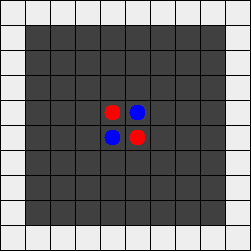
\includegraphics[width=0.4\linewidth]{pics/reversi_original_map.png}
	\captionof{figure}[Bsp. 1 Reversi Karte]{Originales Spielfeld Reversi}
	\label{fig:reversi_original_map}
\end{minipage}
\\

\vspace{1em}
\begin{minipage}{\linewidth}
	\centering
	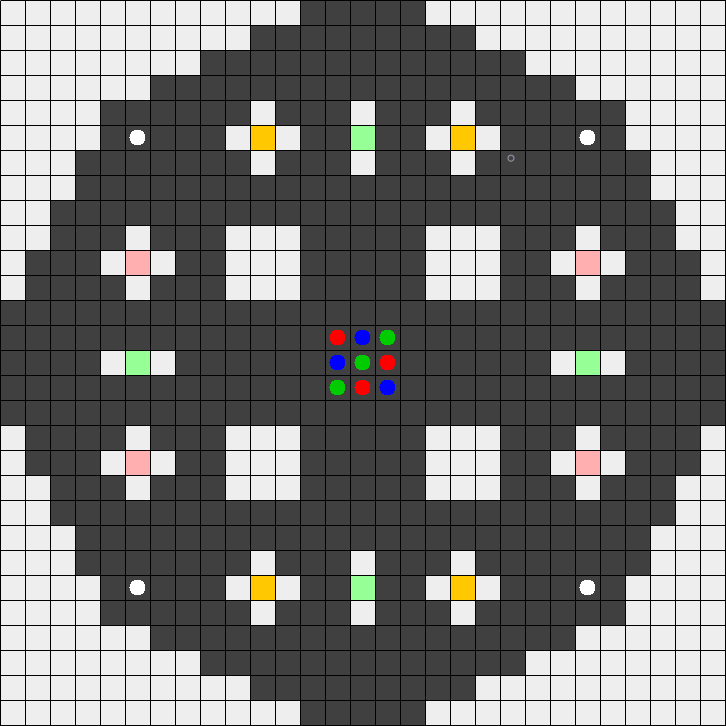
\includegraphics[width=0.7\linewidth]{pics/reversixt_circle_map.png}
	\captionof{figure}[Bsp. 2 ReversiXT Circle Karte]{Spielfeld ReversiXT}
	\label{fig:reversixt_circle_map}
\end{minipage}
\\

Jedem Spieler wird zu Beginn eine Farbe und die dazugehörigen Spielsteine zugewiesen. Das Spielprinzip ist es dann von den eigenen Steinen aus über die der Gegner auf ein freies Feld zu legen, wodurch die eingeschlossenen gegnerischen Steine eingefärbt werden und den Besitzer wechseln. Das bedeutet, dass zwischen dem eigenen Stein und dem freien Feld immer mindestens ein gegnerischer liegen muss. Es kann generell in jede Richtung, horizontal, vertikal und diagonal gezogen werden.
% Bsp. einfärben

Die abgewandelte Variante bietet eine weitere Besonderheit bei der Möglichkeit einen gültigen Zug durchzuführen in Form von sogenannten Überschreibsteine. Diese erlauben es nicht nur auf freie Felder zu legen, sondern auch auf eigene oder gegnerische Steine, um diese einzunehmen, sofern es sich um einen ansonsten regelkonformen Spielzug handelt. Wie viele dieser Steine jeder Spieler zu Beginn zur Verfügung hat, wird vom Ersteller der Karte vorgeschrieben. Es ist jedoch möglich (abhängig vom Spielfeld) zusätzliche dieser Steine im Laufe der Runde zu erhalten, worauf im Weiteren noch genauer eingegangen wird. 
%Bsp. Überschreibsteine

Außerdem können ReversiXT Karten besondere Felder enthalten, die ausgelöst werden sobald ein Spieler das erste Mal darauf zieht. Dazu gehören die Bonusfelder, die dem Spieler die Wahl zwischen einer zusätzlichen Bombe oder eines Überschreibsteins gibt (In Abbildung \ref{fig:reversixt_circle_map} in gelb dargestellt). Setzt ein Spieler auf ein Inversionsfeld werden die Farben der Spieler um eins verschoben, wodurch bspw. Spieler 2 die Steine von Spieler 1, Spieler 3 die von Spieler 2 und Spieler 1 die von Spieler 3 erhält (in Abbildung \ref{fig:reversixt_circle_map} in rosa). Ein Wahlfeld gibt einem Spieler die Möglichkeit seine Steine gezielt mit denen eines Gegners zu tauschen, allerdings kann auch darauf verzichtet werden indem mit den eigenen Steinen \glqq getauscht\grqq{} wird (In Abbildung \ref{fig:reversixt_circle_map} in grün). Als letzte Art von Sonderfeldern sind die Extensionfelder zu nennen, die für alle Spieler als gegnerisches Felder gelten. Dies bedeutet, dass zu jeder Zeit Überschreibsteine darauf gelegt werden dürfen, auch wenn dadurch keine Steine eingeschlossen werden (In Abbildung \ref{fig:reversixt_circle_map} als weiße Steine dargestellt). Ansonsten können diese wie normale Felder behandelt werden.

Eine andere Eigenart von ReversiXT sind die Transitionen, die wie eine Art Portal betrachtet werden können. Sie erlauben es in Richtung von normalerweise nicht bespielbaren Felder zu ziehen, um an einer andere Stelle der Karte (das andere Ende der Transition) herauszukommen. Diese sind ebenfalls optional und können vom Ersteller des jeweiligen Spielfelds gezielt gesetzt werden. Dadurch können Karten bspw. in einzelne Bereiche eingeteilt werden, die nur über Transitionen erreicht werden können, wie es in Abbildung \ref{fig:reversixt_islands_map} dargestellt wird. Die Transitionen werden hierbei durch gelben Linien repräsentiert und bestehen aus einem Ein- und Ausgangsfeld sowie einer Richtung in die diese Transition gültig ist. Ebenso ist zu beachten, dass diese immer in beide Richtungen genutzt werden können.
%Beispiel Zug mit Transition?

\vspace{1em}
\begin{minipage}{\linewidth}
	\centering
	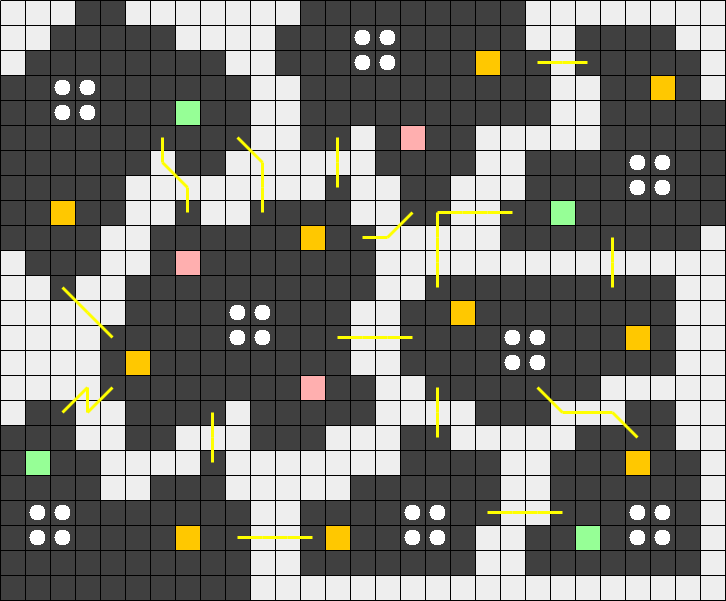
\includegraphics[width=0.7\linewidth]{pics/reversixt_islands_map.png}
	\captionof{figure}[Bsp. 3 ReversiXT Islands Karte]{Spielfeld mit Transitionen}
	\label{fig:reversixt_islands_map}
\end{minipage}
\\


Das Spiel endet sobald kein Spieler mehr einen gültigen Zug machen kann. In der herkömmlichen Version wird an dieser Stelle der Gewinner ermittelt, indem die Anzahl der Steine der Spieler in deren Farbe verglichen wird und derjenige gewinnt, der die meisten einfärben konnte. ReversiXT erweitert das Spielprinzip um eine weiter Spielphase, in der Bomben geworfen werden können. Die Anzahl wie viele Bomben jeder Spieler besitzt sowie deren Stärke wird zu Beginn der Partie festgelegt und kann je nach Spielfeld variieren. Bomben der Stärke zwei zerstören bspw. das Feld an dem sie platziert werden sowie alle Felder in einem Radius von zwei und können somit eine wertvolle Ressource darstellen, da sie gezielt auf die gegnerischen Steine eingesetzt werden können. Nach dieser Phase wird der Sieger wie im klassischen Reversi bestimmt.


\newpage
% ----------------------------------------------------------------------------------
% Kapitel: Allgemeine Informationen
% ----------------------------------------------------------------------------------
\section{Allgemeine Informationen}
Wie in Kapitel \ref{kap:Einleitung} erwähnt wurde das Projekt in einer Kleingruppe von drei Studierenden durchgeführt, weshalb in diesem Kapitel darauf eingegangen wird, wer Teil der Gruppe 05 war, welche Vorkenntnisse vorhanden waren, wie kommuniziert wurde sowie welche technische Mittel verwendet wurden (Soft- und Hardware). Dies soll einen Einblick gewähren, auf welcher Basis das Projekt umgesetzt wurde.

\subsection{Team und Kommunikation}
Die Mitglieder der Gruppe 05 waren Simon Melcher, Robin Jahn und Alexander Wess, die sich alle im vierten Semester ihres Informatik Studiums befanden.

Wichtiges Vorwissen wurde vor allem aus den Fächern Programmieren 2 und Algorithmen und Datenstrukturen von den Studierenden mitgebracht. Dort wurde u. a. anhand von Java die Objektorientierte Programmierung vermittelt, anhand dieser dann verschiedenste Algorithmen in anderen Modulen besprochen und eigene Projekte durchgeführt wurden. Außerdem wurde ein Grundverständnis von Komplexität von Algorithmen mitgebracht, wodurch stärker auf Performance geachtet werden konnte und Einschätzungen getroffen werden konnten, welche Datenstruktur an welcher Stelle sinnvoll war.
%evtl noch aufteilen und genauer?

Neben der wöchentlichen Vorlesung und Übung der Veranstaltung, wurde jede Woche eine Besprechung mit allen Mitgliedern abgehalten. In dieser wurden die Themen der vergangenen Woche diskutiert, das Team auf dem laufenden gehalten wie die Aufgaben umgesetzt wurden und Arbeit aufgeteilt. Zusätzlich wurde über eine gemeinsame WhatsApp Gruppe kommuniziert, in der Fragen gestellt werden konnten und organisatorisches vereinbart wurde.


\vspace{1em}
\begin{table}[!h]
	\centering
	\begin{tabular}{|l|l|l|l|}
		\hline
		\textbf{Simon Melcher} & \textbf{Robin Jahn} & \textbf{Alexander Wess} & \textbf{als Gruppe}\\
		\hline
		1 & 2 & 3\\
		\hline
		4 & 5 & 6\\
		\hline
		7 & 8 & 9\\
		\hline
	\end{tabular}
	\caption{Aufgabenverteilung}
	\label{tab:tasks}
\end{table}

\subsection{Technische Daten}
In diesem Abschnitt soll auf die verwendeten technischen Mittel eingegangen werden. Das Projekt wurde in der Programmiersprache Java in der 11ten Version umgesetzt, da zum einen darin bereits die meiste Erfahrung gesammelt werden konnte. Zum anderen konnten die gängigen Vorteile dieser Programmiersprache genutzt werden, wie z. B. die automatische Speicher- und Heap-Verwaltung oder die Möglichkeit mit \glqq Call by Reference\grqq{} zu arbeiten.
Zu Beginn legte sich die Gruppe fest einheitlich die Entwicklungsumgebung IntelliJ IDEA der Version 2021.3.3 von JetBrains zu nutzen. Der Vorteil davon war u. a., dass diese bereits eine gute Anbindung an Git besitzte und somit das Arbeiten in einem gemeinsam Repository signifikant erleichterte.
Als Betriebssystem wurde hauptsächlich Windows 10 der Version 21H2 verwendet. Außerdem wurde von Robin Jahn eine virtuelle Maschine eingerichtet, die das Unix Betriebssystem Ubuntu simulierte, um Tests mit dem Server zu machen, über den im späteren Verlauf der Veranstaltung die Spiele ausgetragen wurden. Dadurch sollte sichergestellt werden, dass der entwickelte Client fehlerlos über ein Linux Betriebssystem ausgeführt werden konnte und die Kommunikation mit dem Server reibungslos funktionierte.

\newpage
% ----------------------------------------------------------------------------------
% Kapitel: Spielfeldbewertung
% ----------------------------------------------------------------------------------
\section{Spielfeldbewertung}
Versuchen Sie eine \emph{weiche} Überleitung in dieses Kapitel zu formulieren, indem Sie kurz beschreiben, was den Leser in diesem Kapitel erwartet und warum das für die entstehende K.\,I.\ interessant ist.

\subsection{Bestandteile}\label{kap:Heuristik_Beschreibung}
Eine mögliche Heuristik zur Spielfeldbewertung ist die eigene Flexibilität in Bezug auf durchführ"-bare Spielzüge (in diesem Kontext auch als "Mobilität" bezeichnet), die sich aus der jeweiligen Situation ergeben. Hierbei ist der Grundgedanke der, dass der Spieler nicht nur darauf achtet möglichst viele Steine auf dem Feld zu haben bzw. beim Tätigen eines Spielzugs möglichst viele Steine einzufärben (Greedy-Verfahren), sondern ebenfalls zu berücksichtigen wie viele Optionen er hat das Spiel weiterzuführen. Mehr valide Züge als die Gegner zu haben ist dementsprechend von Vorteil. Dadurch soll sichergestellt werden, dass die eigene Strategie weiterverfolgt werden kann und nicht der Gegner den Spielverlauf vorgibt oder man zu \glqq schlechten\grqq{} Zügen gezwungen wird.

Die zuvor beschriebene Situation ist in Abbildung \ref{fig:example_heuristics_flexibility_simple} zu sehen. Der Spieler mit den blauen Steinen hat zwar mehr eingefärbt, kann jedoch nicht mehr ziehen (sofern keine Überschreibsteine verfügbar sind) und muss abwarten, was der Spieler mit den roten Steinen als nächstes macht. Dieser kann hingegen frei entscheiden in welche Richtung die Karte als Nächstes bespielt werden soll, da er in jede Richtung ziehen kann.

\vspace{1em}
\begin{minipage}{\linewidth}
	\centering
	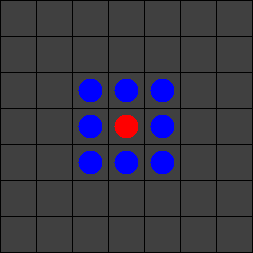
\includegraphics[width=0.3\linewidth]{pics/heuristics_flexibility_simple.png}
	\captionof{figure}[Bsp. 1 Heuristik Flexibilität]{Situation Blau kann nicht mehr ziehen}
	\label{fig:example_heuristics_flexibility_simple}
\end{minipage}
\\

Jedoch bringt dieses Verfahren auch Nachteile mit sich, da das Ziel des Spiels, am Ende der Partie die meisten Steine auf dem Spielfeld zu haben, vernachlässigt wird. Somit gestaltet es sich viel mehr am Anfang bis zur Mitte einer Runde als sinnvoll bzw. sollte noch mit anderen Verfahren kombiniert werden.


Ein weiterer Ansatz der Spielfeldbewertung ist die \glqq Sicherheit\grqq{} der einnehmbaren Felder. In diesem Fall soll darauf geachtete werden, ob und wie leicht die jeweiligen Felder vom Gegner eingefärbt werden können. Folglich muss hierbei überprüft werden, ob ein Feld, nachdem es das erste Mal besetzt wird, überhaupt noch einmal den Besitzer wechseln kann oder aus wie vielen Richtungen die Gegner noch Möglichkeiten haben, dieses Feld zurückzugewinnen. Zusätzlich soll die Anzahl der Wege, in die von diesem Feld aus gezogen werden kann, einkalkuliert werden. Diese Analyse kann anhand eines Punktesystems realisiert werden.


Das naheliegendste Beispiel für ein solches sicheres Feld ist eine Ecke wie in Abbildung \ref{fig:example_heuristics_safe_fields_corner} dargestellt. Dieser Stein kann weder horizontal noch vertikal oder diagonal von einem Gegner eingefärbt werden und stellt somit eine wertvolle Position dar. %Ergänzen in wie viele Richtungen gezogen werden kann

%ToDo: Pfeile einfügen, besseres Beispiel? Also mit maximalen Wert -> noch eine Richtung mehr0
\vspace{1em}
\begin{minipage}{\linewidth}
	\centering
	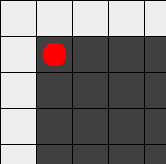
\includegraphics[width=0.3\linewidth]{pics/heuristics_safe_fields_corner.png}
	\captionof{figure}[Bsp. 1 Heuristik sichere Felder]{Nicht einnehmbares Feld mit vielen 		Zugmöglichkeiten}
	\label{fig:example_heuristics_safe_fields_corner}
\end{minipage}
\\

Abbildung \ref{fig:example_heuristics_safe_fields_dead_end} zeigt eine andere Situation, in der das Feld zwar ebenfalls nicht mehr eingenommen werden kann, jedoch auch nur eine Richtung (nach Unten) als Zugmöglichkeit bietet.

\vspace{1em}
\begin{minipage}{\linewidth}
	\centering
	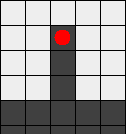
\includegraphics[width=0.3\linewidth]{pics/heuristics_safe_fields_dead_end.png}
	\captionof{figure}[Bsp. 2 Heuristik sichere Felder]{Nicht einnehmbares Feld mit wenigen Zugmöglichkeiten}
	\label{fig:example_heuristics_safe_fields_dead_end}
\end{minipage}
\\

Ein Feld, das sich am Rand der Karte befindet, kann zwar eingenommen werden, jedoch sind die Möglichkeiten beschränkt, da es lediglich vertikal von gegnerischen Spielern eingefärbt werden kann, wie es in Abbildung \ref{fig:example_heuristics_safe_fields_outer_side} zu sehen ist. Gleichzeitig eröffnet es Möglichkeiten in fünf Richtungen den nächsten Spielzug durchzuführen.

%ToDo: Pfeile einfügen
\vspace{1em}
\begin{minipage}{\linewidth}
	\centering
	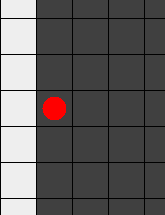
\includegraphics[width=0.3\linewidth]{pics/heuristics_safe_fields_outer_side.png}
	\captionof{figure}[Bsp. 3 Heuristik sichere Felder]{Beschränkt einnehmbares Feld}
	\label{fig:example_heuristics_safe_fields_outer_side}
\end{minipage}
\\

Wenn jedoch keine Seite durch das Ende der Karte geschützt ist, ist dieses Feld von allen Seiten für den Gegner erreichbar und kann mit einer niedrigeren Priorität berücksichtigt werden. In Abbildung \ref{fig:example_heuristics_safe_fields_middle} wird dies durch ein Feld inmitten der Spielfläche verdeutlicht.

%ToDo: Pfeile einfügen
\vspace{1em}
\begin{minipage}{\linewidth}
	\centering
	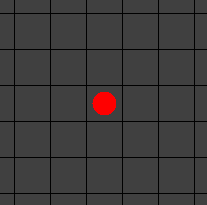
\includegraphics[width=0.3\linewidth]{pics/heuristics_safe_fields_middle.png}
	\captionof{figure}[Bsp. 4 Heuristik sichere Felder]{Voll einnehmbares Feld}
	\label{fig:example_heuristics_safe_fields_middle}
\end{minipage}
\\

Die Schwierigkeit dieser Heuristik besteht darin, dass die Sonderregeln von ReversiXT nicht vernachlässigt werden dürfen. Ein vermeintlich sicheres Feld (z. B. eine Ecke), kann durch Transitionen gar kein uneinnehmbares Feld sein und muss auch als dieses behandelt werden. Ebenso können Überschreibsteine diesen Effekt hervorrufen.

\subsection{Implementierung}\label{kap:Heurisitk_Implementierung} %Vorübergehend in zwei Unterkapitel getrennt. Also Idee der Heuristik und Umsetzung
Zur Umsetzung der Spielfeldbewertung hinsichtlich der Mobilität wurde die Anzahl der eigenen möglichen Spielzüge mit der der Gegnern verglichen. Hierfür wurde ein Durchschnittswert aus allen durchführbaren gegnerischen Zügen und der Anzahl der Kontrahenten ermittelt, der daraufhin zur Gegenüberstellung verwendet wurde.

%%Bsp einfügen. Wird das aktuell richtig dargestellt?

Die Analyse zur Sicherheit der Felder bzw. deren Wert wurde anhand eines Punktesystems realisiert. Hierbei sollte jedem Feld eine Zahl zugeordnet werden, die auf Basis von einigen Kriterien errechnet wurde und somit darstellte, wie bedeutend dieses ist. Wie bereits in Kapitel \ref{kap:Heuristik_Beschreibung} erwähnt sind zum einen die Möglichkeiten der Gegner zur Eroberung des Feldes als auch die daraus ausgehenden Wege maßgebend. Das Endergebnis einer solchen Berechnung ist in Abbildung \ref{fig:example_heuristics_implementation_field_values_matrix} zu sehen. Hier ist deutlich zu erkennen, dass Felder in den Ecken oder am Rand höher beziffert wurden als welche in der Mitte der Karte. Darüber hinaus wurde darauf geachtet, dass die wertvollen Felder auch erreicht werden können, indem die angrenzenden Bereiche mit negativen Zahlen gewichtet wurden. Dadurch soll signalisiert werden, dass diese Felder gemieden werden sollten, da sie dem Spieler die Chance verwehrt auf eines der vorteilhaften Felder zu ziehen und nur dem Gegner die Gelegenheit dafür geben würde. 

\vspace{1em}
\begin{minipage}{\linewidth}
	\centering
	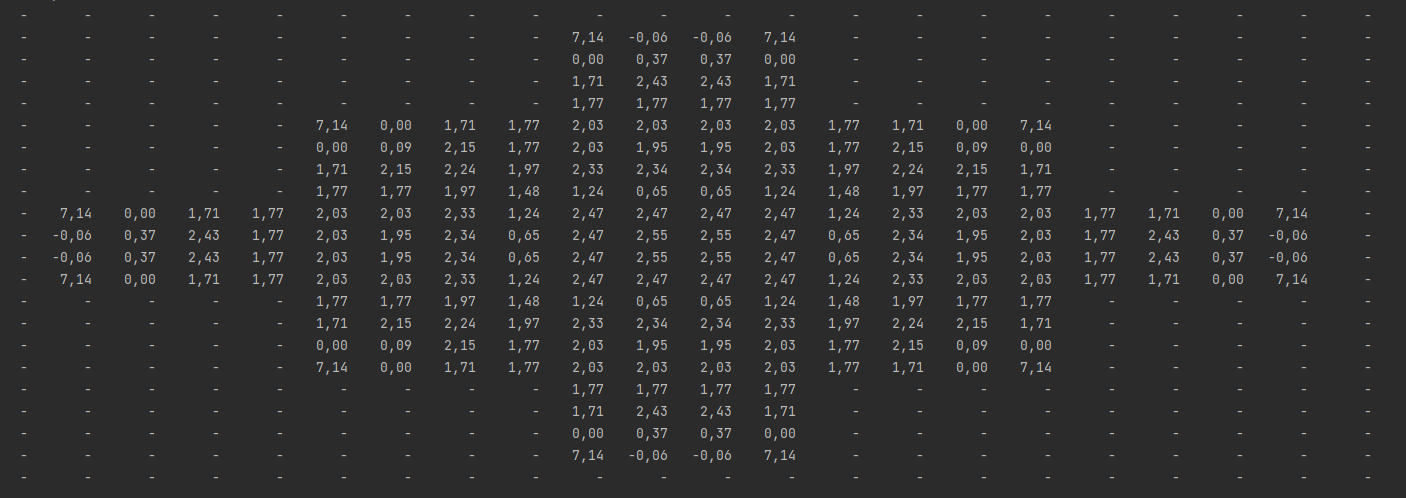
\includegraphics[width=0.8\linewidth]{pics/heuristics_implementation_field_values_matrix.png}
	\captionof{figure}[Bsp. 1 Heuristik Implementierung Bewertung Felder]{Spielfeld mit Punktzahl zur Bewertung der Felder}
	\label{fig:example_heuristics_implementation_field_values_matrix}
\end{minipage} 
 

\newpage
% ----------------------------------------------------------------------------------
% Kapitel: Fazit
% ----------------------------------------------------------------------------------
\section{Fazit}
Beschreiben Sie in diesem Abschnitt u.a.\ was Ihnen an diesem Fach gefallen hat und welche Verbesserungsvorschläge Sie für künftige Veranstaltungen haben. Was konnten Sie dazulernen, in welchen Bereichen haben Sie sich verbessert. Welche Problemsituationen gab es während der Projekterstellung, wie sind Sie diese angegangen und wie haben Sie diese gelöst. Was haben Sie evtl.\ vermisst.


\newpage
% ----------------------------------------------------------------------------------
% Kleine Einführung in LaTeX-Elemente
% ----------------------------------------------------------------------------------
\section{\LaTeX-Elemente}
Dieser Abschnitt soll nicht Bestandteil des Projektberichtes sein, sondern beinhaltet lediglich einige Informationen über \LaTeX-Distributionen, Editoren und \LaTeX-Elemente, die Ihnen beim Einstieg in das \LaTeX-Textsatzsystem helfen sollen.

\subsection{\LaTeX-Distributionen nach Betriebssystemen}

\subsubsection{\LaTeX-Distributionen}
Folgende Haupt-\LaTeX-Distributionen stehen Ihnen zur Verfügung:
\begin{itemize}
  \item Windows:\quad \texttt{MiKTeX}\quad Webseite:\quad\url{http://www.miktex.org}
  \item Linux/Unix:\quad \texttt{TeX Live}\quad Webseite:\quad\url{http://tug.org/texlive/}
  \item Mac OS:\quad \texttt{MacTeX}\quad Webseite:\quad\url{http://www.tug.org/mactex/}
\end{itemize}

\subsubsection{\LaTeX-Editoren}
Auf folgenden Webseiten können Sie einige hilfreiche \LaTeX-Editoren finden:
\begin{itemize}
  \item Windows/Linux/Mac OS: \url{http://www.xm1math.net/texmaker/}
  \item Windiws: \url{http://www.texniccenter.org/}
  \item Mac OS: \url{http://pages.uoregon.edu/koch/texshop/}
\end{itemize}

Falls bei den oben genannten Editoren kein passender vorhanden war, findet sich auf Wikipedia eine Zusammenstellung vieler weiterer \LaTeX-Editoren:\\[1em]
\hspace*{3cm}\url{https://en.wikipedia.org/wiki/Comparison_of_TeX_editors}


\subsection{Unterabschnitt}\label{Kap:Minipage}
Zum Einfügen eines Bildes, siehe Abbildung \ref{fig:reversi01}, wird die \textit{minipage}-Umgebung genutzt, da die Bilder so gut positioniert werden können.

\vspace{1em}
\begin{minipage}{\linewidth}
	\centering
	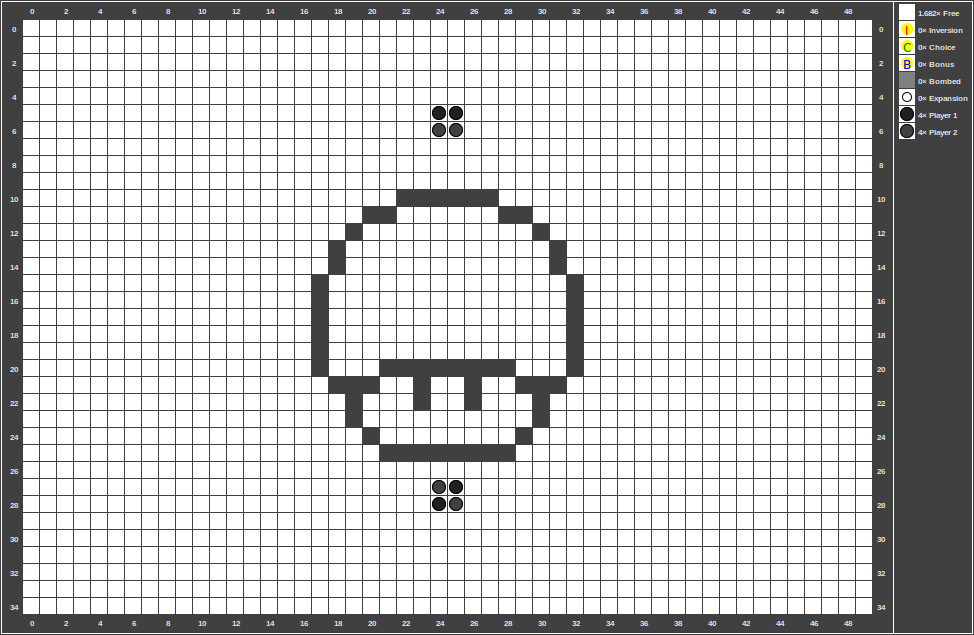
\includegraphics[width=0.6\linewidth]{pics/gamefield01.png}
	\captionof{figure}[Spielfeld 01]{Unbespieltes Spielfeld\footnotemark }
	\label{fig:reversi01}
\end{minipage}
\footnotetext{Diesem Spielfeld wurden noch keine Spieler zugewiesen (daher die dunklen Spielsteine)}

Nachdem das Spielt gestartet wurde und beide Spielphasen durchlaufen wurden, siegt schließlich der Spieler mit der Farbe rot.

\vspace{1em}
\begin{minipage}{\linewidth}
	\centering
	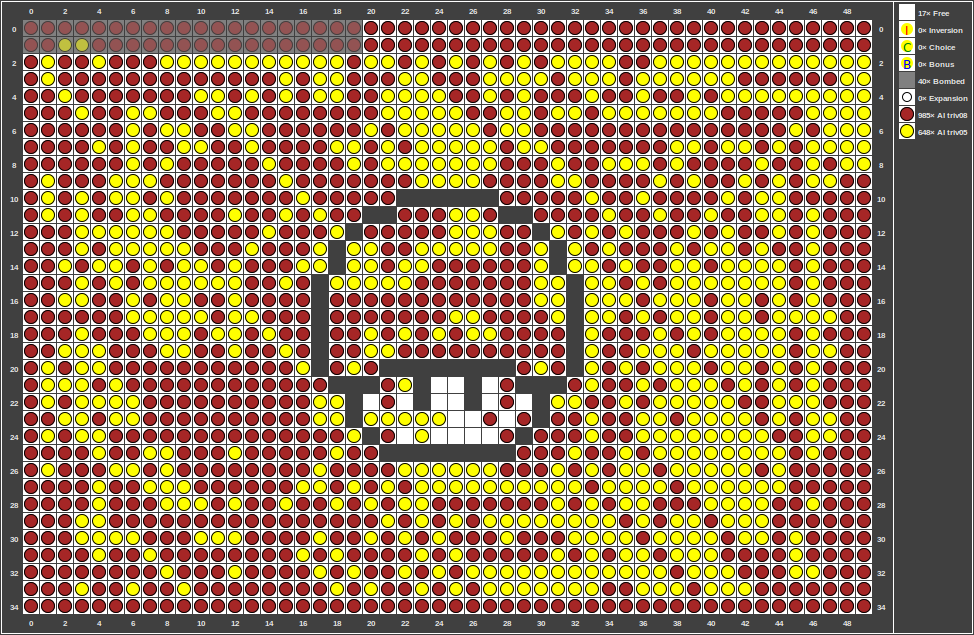
\includegraphics[width=0.6\linewidth]{pics/gamefield02.png}
	\captionof{figure}[Spielfeld 02]{Finales Spielfeld\footnotemark }
	\label{fig:reversi2}
\end{minipage}
\footnotetext{Das Spielfeld nach der Zug- und Bombenphase. Spieler rot gewinnt eindeutig.}

\subsection{Tabellen}
In diesem Abschnitt wird eine Tabelle (siehe Tabelle \ref{tab:beispiel}) dargestellt.

\vspace{1em}
\begin{table}[!h]
	\centering
	\begin{tabular}{|l|l|l|}
		\hline
		\textbf{Name} & \textbf{Name} & \textbf{Name}\\
		\hline
		1 & 2 & 3\\
		\hline
		4 & 5 & 6\\
		\hline
		7 & 8 & 9\\
		\hline
	\end{tabular}
	\caption{Beispieltabelle}
	\label{tab:beispiel}
\end{table}


\subsection{Auflistung}
Für Auflistungen wird die \texttt{enumerate}- oder \texttt{itemize}-Umgebung genutzt.

\begin{itemize}
	\item Nur
	\item ein
	\item Beispiel.
\end{itemize}

\subsection{Listings}
\subsection{Listings}
Zuletzt sehen Sie in Listing \ref{lst:maxTeilsumZweiD} ein Beispiel für das Einbinden von Quellcode mit Syntax-Highlighting.

\vspace{1em}
\lstinputlisting[caption=Brute Force-Ansatz für das MaxTeilsum2D-Problem, label=lst:maxTeilsumZweiD,basicstyle=\ttfamily\scriptsize]{code/maxTeilsum2DBruteForce.txt}

\subsection{Selbstgestaltete Abbildungen}
Mithilfe des Paketes \texttt{tikz} können sehr schöne Abbildungen (z.\,B.\ Automaten, Graphen etc.) direkt in \LaTeX generiert werden. Viele Beispiele dazu finden Sie auf folgender Webseite:\\[1em]
\hspace*{3cm}\url{http://www.texample.net/tikz/}.

\subsection{Tipps}
Die Quellen befinden sich in der Datei \textit{quellen.bib}. Eine Buch- und eine Online-Quelle sind beispielhaft eingefügt. [Vgl. \cite{buch}, \cite{online}]

\pagebreak

% ----------------------------------------------------------------------------------------------------------
% Kapitel
% ----------------------------------------------------------------------------------------------------------
\section{Kapitel}
Lorem ipsum dolor sit amet.

\subsection{Unterkapitel}
Lorem ipsum dolor sit amet, consetetur sadipscing elitr, sed diam nonumy eirmod tempor invidunt ut labore et dolore magna aliquyam erat, sed diam voluptua. At vero eos et accusam et justo duo dolores et ea rebum. Stet clita kasd gubergren, no sea takimata sanctus est Lorem ipsum dolor sit amet. Lorem ipsum dolor sit amet, consetetur sadipscing elitr, sed diam nonumy eirmod tempor invidunt ut labore et dolore magna aliquyam erat, sed diam voluptua. At vero eos et accusam et justo duo dolores et ea rebum. Stet clita kasd gubergren, no sea takimata sanctus est Lorem ipsum dolor sit amet.

\subsection{Unterkapitel}
Lorem ipsum dolor sit amet, consetetur sadipscing elitr, sed diam nonumy eirmod tempor invidunt ut labore et dolore magna aliquyam erat, sed diam voluptua. At vero eos et accusam et justo duo dolores et ea rebum. Stet clita kasd gubergren, no sea takimata sanctus est Lorem ipsum dolor sit amet. Lorem ipsum dolor sit amet, consetetur sadipscing elitr, sed diam nonumy eirmod tempor invidunt ut labore et dolore magna aliquyam erat, sed diam voluptua. At vero eos et accusam et justo duo dolores et ea rebum. Stet clita kasd gubergren, no sea takimata sanctus est Lorem ipsum dolor sit amet.
\pagebreak

% ----------------------------------------------------------------------------------------------------------
% Literatur
% ----------------------------------------------------------------------------------------------------------
\renewcommand\refname{Quellenverzeichnis}
\bibliographystyle{alpha}
\bibliography{quellen}
\pagebreak

% ----------------------------------------------------------------------------------------------------------
% Anhang
% ----------------------------------------------------------------------------------------------------------
\pagenumbering{Roman}
\setcounter{page}{1}
\lhead{Anhang \thesection}

\begin{appendix}
\section*{Anhang}
\phantomsection
\addcontentsline{toc}{section}{Anhang}
\addtocontents{toc}{\vspace{-0.5em}}

\section{GUI}
Ein toller Anhang.

\subsection*{Screenshot}
\label{app:screenshot}
Unterkategorie, die nicht im Inhaltsverzeichnis auftaucht.

\end{appendix}


\end{document}
